%%%%%%%%%%%%%%%%%%%%%%%%%%%%%%%%%%%%%%%%%%%%%%
%                insertmeeting
% 1) Title (something creative & funny?)
% 2) Date (MM/DD/YYYY)
% 3) Location (ex. Hagerty High School)
% 4) People/Committees Present 
% 5) Picture 
% 6) Start Time & Stop Time (ex. 12:30AM to 4:30PM)
%%%%%%%%%%%%%%%%%%%%%%%%%%%%%%%%%%%%%%%%%%%%%%
\insertmeeting 
	{Meeting Example} 
	{01/20/22} 
	{Hagerty High School}
	{Falon, James, Jensen, Nathan, Ritam, Samantha}
	{Images/RobotPics/robot.jpg}
	{2:30 - 4:30}
	
\hhscommittee{Software}
\noindent\hfil\rule{\textwidth}{.4pt}\hfil
\subsubsection*{Goals}
\begin{itemize}
    \item Explore if Vuforia vision systems can be added to our current navigation system.  

\end{itemize} 

\noindent\hfil\rule{\textwidth}{.4pt}\hfil

\subsubsection*{Accomplishments}
Today we looked at the "ConceptVuforiaFieldNavigationWebcam" example from FtcRobotController's external samples. Our plan is to use Vuforia's pre-built tracking systems to figure out where the robot is relative to the center of the field. Like our exisiting localization systems, the Vuforia system places the x-axis parallel to the red alliance wall. This means that we can easily integrate the new camera localization into our existing navigation systems. Attached shows the segment that we will use in our TeamCode to find the location of the robot. 

\begin{figure}[htp]
\centering
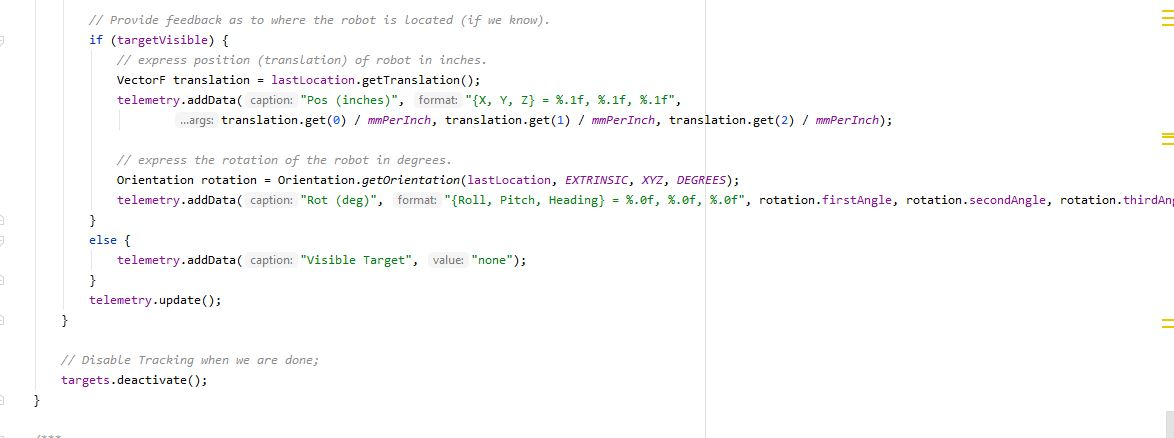
\includegraphics[width=0.95\textwidth, angle=0]{Meetings/January/01-20-22/1.20.22 vuforia localization spot - James Hu.JPG}
\caption{FTC sample code that we plan to incorporate into our code}
\label{fig:012022_1}
\end{figure}


\whatsnext{
\begin{itemize}
    \item Integrate the position from Vuforia into our autonomous movement.
\end{itemize} 
}

